

\subsection{Model Scale}\label{sec:eval_efficiency}

In this section, we investigate the performance of FSDP when dealing with models of different sizes, spanning from 611M to 175B, and make a comparison with DDP~\cite{ddp}.




%\begin{figure}
%    \centering
%    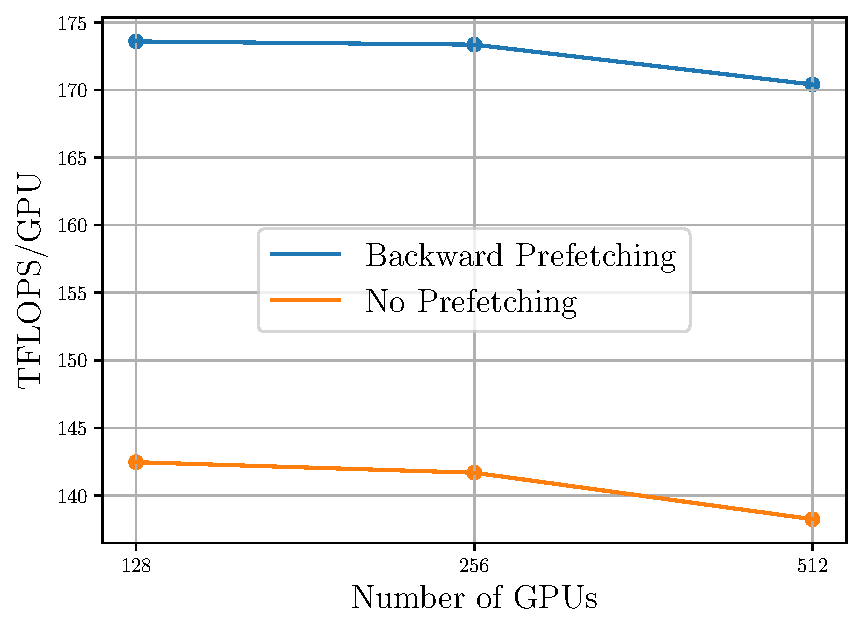
\includegraphics[width=\linewidth]{figure/prefetching_tflops.pdf}
%    \caption{Backward Prefetch On/Off: with 80GB A100, 8 GPUs per Machine}
%    \label{fig:prefetching_tflops}
%\end{figure}

The experimental results on T5 models are displayed in Figure~\ref{fig:mix}~(a). The performance of FSDP and DDP is similar when evaluating 611M and 2.28B models. However, DDP encounters an out-of-memory error when attempting to wrap models larger than 2.28B. In contrast, FSDP can effortlessly accommodate the 11B model and achieve significantly higher TFLOPS by turning on \code{BF16}. These experiments illustrate that practitioners can utilize FSDP for both small and large models, and seamlessly transition across different model configurations.

Then, we conduct additional experiments to measure the acceleration attained through backward pre-fetching. This time we use a larger GPT-175B model, where communication overhead is more prominent. Results are presented in Figure~\ref{fig:mix}~(b), where pre-fetching leads to approximately 18\% speedup, and this TFLOPS gain persists across different GPU cluster sizes. Therefore, for subsequent experiments, we always turn-on backward pre-fetching. 





